\chapter{Технологическая часть}

В данном разделе будет представлена реализация решения поставленной задачи в в формате листинга кода. Также будут указаны требования к ПО и средства реализации, описан пользовательский интерфейс и результаты проведённого тестирования программы.

\section{Требования к ПО}
Были учтены следующие требования к программе:
\begin{enumerate}[label={\arabic*)}]
	\item Программа выводит сообщение об ошибке и генерирует ненулевой код возврата в случае возникновения исключения в процессе выполнения.
	\item Программа выполняет построение изображения сцены из трёхмерных объектов, которые могут представлять из себя многогранники, сферы, или комбинацию из двух объектов одного типа~---~пузырь.
	\item Программа выполняет обработку только многогранников, геометрия которых описана с помощью $obj$ файла, и только сферы, геометрия которых описана аналитическим способом (с помощью указания основных параметров канонического уравнения сферы).
	\item Программа принимает на вход файлы, составленные по правилам, которые описаны ниже.  
	\item Программа может сохранять полученное изображение в $png$ файл.
	\item Программа предоставляет возможность замера времени выполнения при вызове из командной строки.
	\item Программа предоставляет возможность проведения модульного тестирования при вызове из командной строки.
	\item Программа предоставляет возможность изменять положение как отдельного объекта сцены, так и всех объектов сцены одновременно, а именно перемещать объекты, масштабировать их и вращать относительно собственного центра;
	\item Программа предоставляет возможность указать, какое количество потоков должно быть выделено для обработки сцены, и какой будет глубина рекурсивных погружений при работе алгоритма обратной трассировки лучей.
\end{enumerate}

На рисунках \ref{img:idef0-1}~--~\ref{img:idef0-2} представлена функциональная модель программы в нотации $IDEF0$.

\begin{figure}[h!]
    \centering
    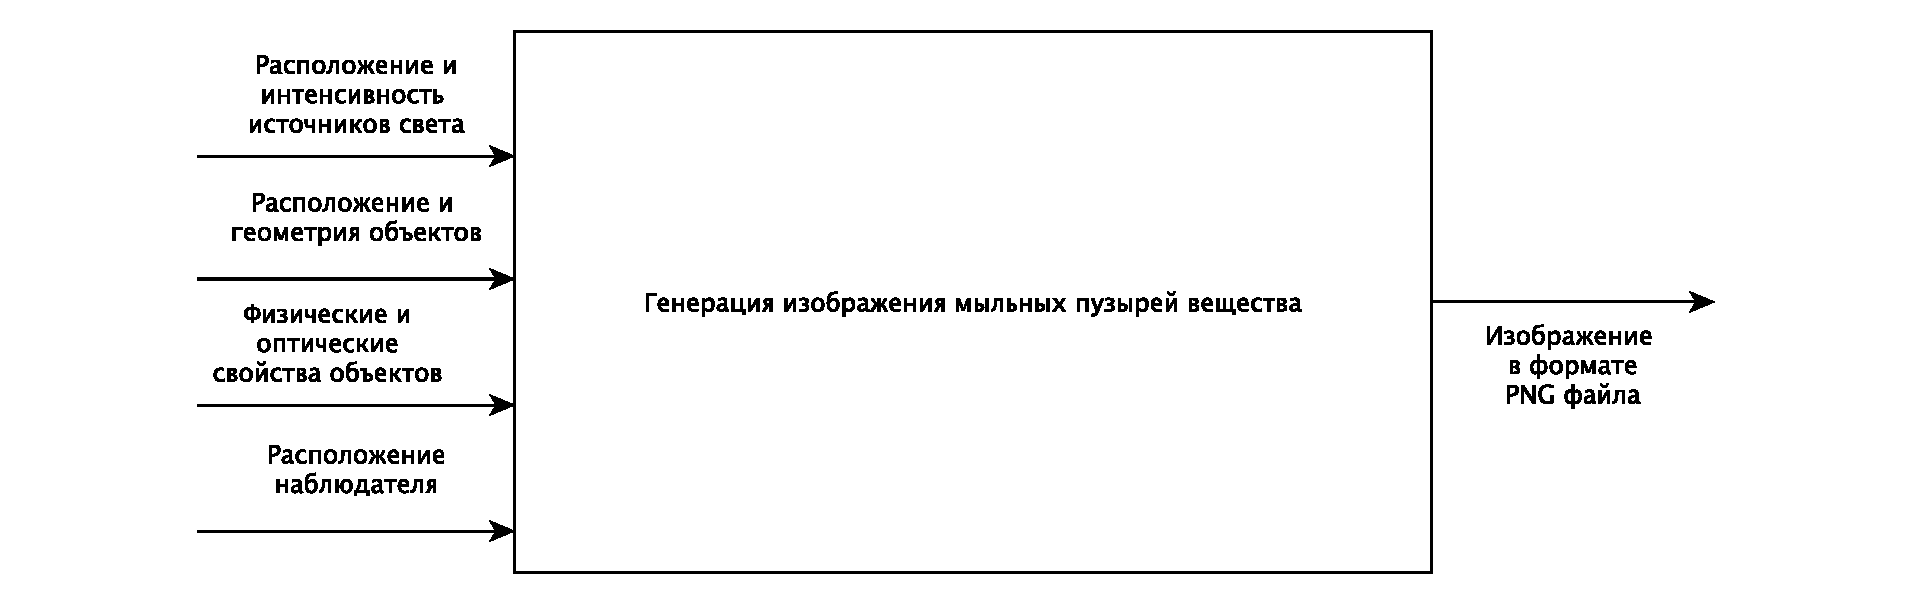
\includegraphics[width=1\linewidth]{idef0-1.pdf}
    \caption{Функциональная модель программы (начало)}
    \label{img:idef0-1}
\end{figure}

\begin{figure}[h!]
    \centering
    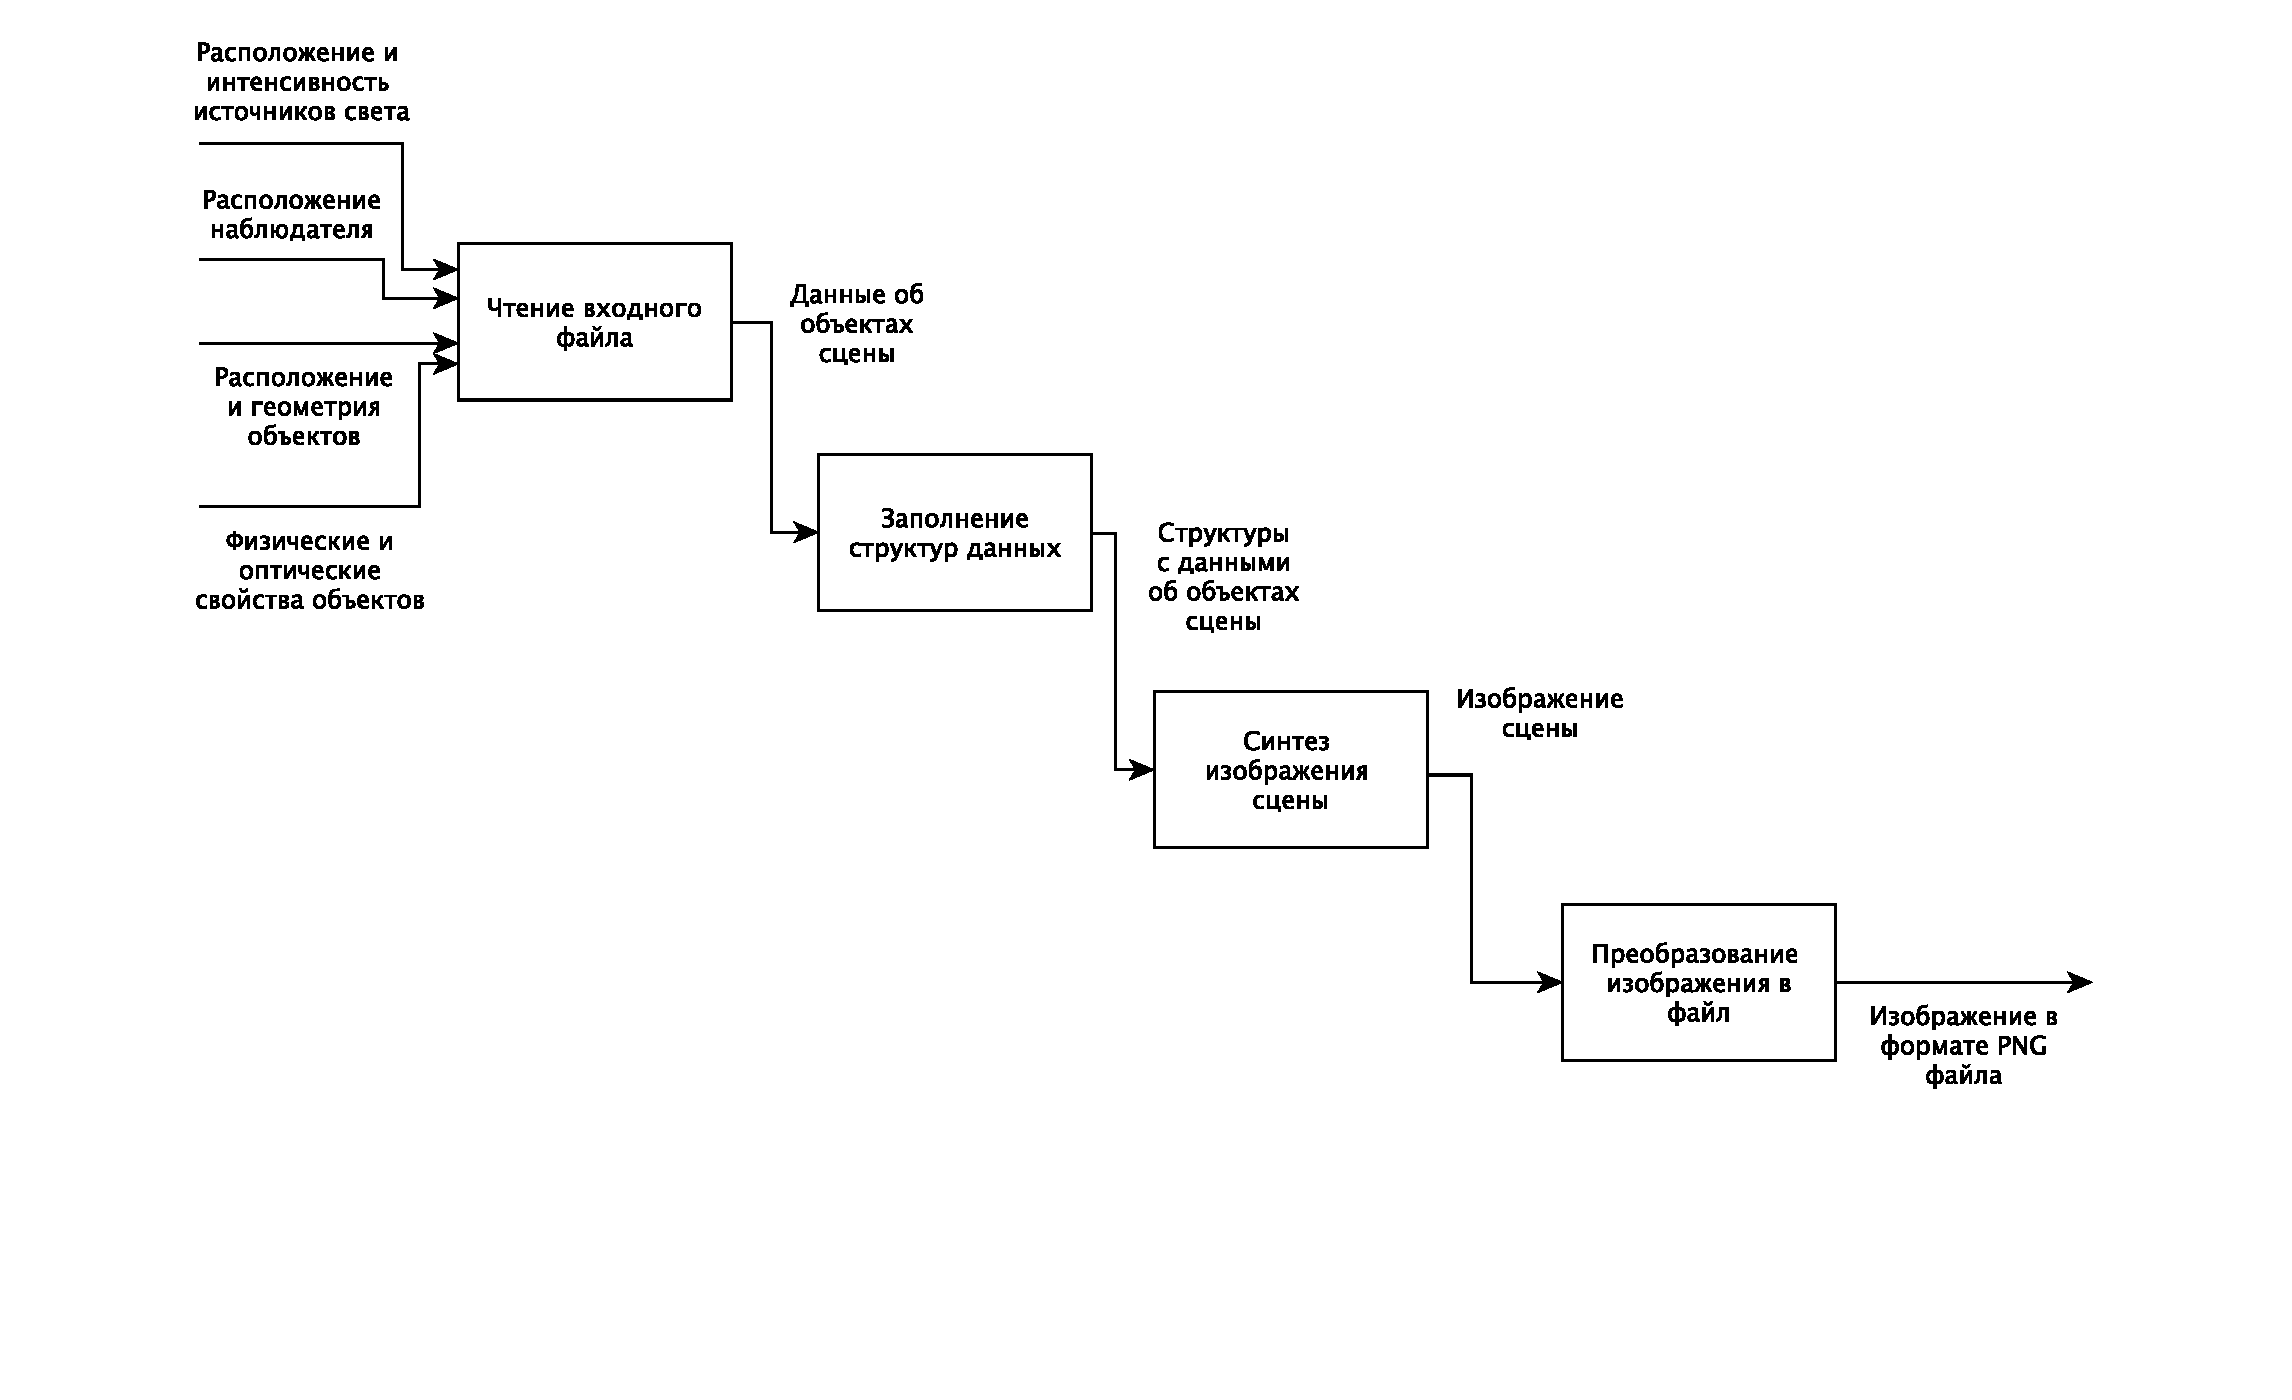
\includegraphics[width=1\linewidth]{idef0-2.pdf}
    \caption{Функциональная модель программы (продолжение рисунка \ref{img:idef0-1})}
    \label{img:idef0-2}
\end{figure}

\section{Требования к входным данным}
Требования ко входному файлу:
\begin{enumerate}[label={\arabic*)}]
	\item На вход принимаются только $txt$ файлы.
	\item Для описания сферы, заданной аналитически, перед указанием непосредственно параметров фигуры, указывается параметр $A$.
	\item Для описания многогранника, заданного при помощи полигональной сетки, перед указанием имени файла с параметрами фигуры, указывается параметр $O$.
	\item Для описания пузыря указывается параметр $B$, после него следует один из вышеуказанных параметров в зависимости от способа описания слоёв.
	\item Для описания источника света указывается параметр $L$, после которого следует информация об источнике света.
\end{enumerate}

Параметры фигур:
\begin{enumerate}[label={\arabic*)}]
	\item Для сферы, заданной аналитически, необходимо указать координаты точки центра, радиус, параметры материала~---~коэффициенты рассеянного, диффузного и зеркального отражения, коэффициенты пропускания и преломления, оптическая плотность, диффузный цвет и цвет бликов.
	\item Для многогранника, заданного при помощи полигональной сетки, необходимо указать имя $obj$ файла, в котором хранится информация о данном многограннике. В одном файле может хранится информация о нескольких многогранниках.
	\item Для пузыря необходимо привести описания двух его слоёв в соответствии с указанными выше правилами. Пузырь может состоять только из двух слоёв одного типа.
\end{enumerate}

\section{Реализация управления из командной строки}
Для автоматизации работы программы необходимо реализовать передачу в программу аргументов командной строки и их распознавание самой программой. Для этого была использована функция $getopt$ \cite{web_item17}, которая последовательно перебирает переданные параметры в программу в соответствии с заданной строкой параметров, содержащей имена параметров и признак наличия передаваемого значения (символ двоеточие).

Были предусмотрены следующие флаги:

\begin{itemize}
	\item флаг «$-d$» определяет значение глубины рекурсивных погружений, за именем флага следует положительное целочисленное значение;
	\item флаги «$-i$», «$-o$» определяют имена входного и выходного файлов соответственно, за именем флага следует строка с именем файла;
	\item флаг «$-n$» определяет количество выделяемых потоков, за именем флага следует положительное целочисленное значение;
	\item флаг «$-r$» определяет угол поворота сцены вокруг выбранной оси, за именем флага следует целочисленное значение;
	\item флаг «$-m$»~---~указание программе о том, что проводятся замеры времени работы, при этом обязательно наличие параметров «$-d$» и «$-i$», а «$-o$» становится необязательным, так как полученное изображение в данном случае не используется;
	\item флаг «$-t$»~---~указание программе о том, что проводится модульное тестирование, при этом все остальные параметры необязательны.
\end{itemize}

При стандартном запуске программы, когда важно полученное изображение, передача параметров «$-d$», «$-i$» и «$-o$» является обязательной, в случае отсутствия обязательных параметров программой генерируется ненулевой код возврата.

\section{Средства реализации}
В качестве языка программирования для разработки ПО был выбран язык программирования $C++$ \cite{web_item4}. Данный выбор обусловлен наличием необходимого функционала для работы с наборами объектов и проведения исследования по замеру времени выполнения. Также был выбран фреймворк $Qt$ \cite{web_item2} в связи с наличием необходимых для работы с компьютерной графикой библиотек и встроенных средств. Для передачи сведений об объектах сцены в программу использовались файлы с расширением $txt$, как имеющие наибольшую гибкость для формализации ввода. 

Для хранения информации о многогранниках, заданных при помощи полигональной сетки, были использованы $obj$ файлы. Данный выбор обусловлен тем, что $obj$ является одним из самых популярных форматов передачи трёхмерной компьютерной геометрии \cite{web_item18}, позволяет хранить информацию о текстурах в отдельном $mtl$ файле в отличие от некоторых аналогов, например, $stl$ файлов, и имеет широкую поддержку экспорта и импорта программного обеспечения САПР. Для хранения полученного изображения был выбран формат $png$, так как среднеквадратическая ошибка~---~среднее различие в квадрате между идеальным и фактическим пиксельными значениями~---~для, например, $jpeg$ файлов на больших изображениях гораздо больше, чем у $png$ файлов \cite{web_item19}, и качество изображения формата $png$ не меняется при любой степени сжатия.

\section{Реализация разработанного ПО}
В листингах \ref{code:1}~--~\ref{code:4} представлена реализация алгоритма обратной трассировки лучей с учётом интерференции света, в листинге \ref{code:5} представлена реализация поиска первого пересечения луча с объектом сцены, в листинге \ref{code:6} представлена реализация поиска пересечения луча с многогранником, в листинге \ref{code:7} представлена реализация поиска пересечения луча с многоугольником, в листинге \ref{code:8} представлена реализация поиска пересечения луча со сферой, в листингах \ref{code:9}~--~\ref{code:10} представлена реализация проверки принадлежности точки многоугольнику.

\begin{code}
\caption{Листинг функции, реализующей алгоритм обратной трассировки лучей с учётом интерференции света (начало)}
\label{code:1}
\begin{minted}{c++}
QColor Drawing::castRay(const sight_t& sight, const int& depth)
{
    double intensity = 0.0;
    double specIntensity = 0.0;

    std::tuple<bool, double, QVector3D, int> res = sceneIntersect(sight);
    if (depth > this->depth)
        return Qt::black;
    if (!std::get<0>(res))
            return bgc;

    double t = std::get<1>(res);
    QVector3D norm = std::get<2>(res);
    int closest = std::get<3>(res);
    QVector3D cam = sight.start;
    QVector3D dir = sight.dir;
    QVector3D intersection = cam + dir * t;
    double reflectK = 0.0;
\end{minted}
\end{code}

\newpage

\begin{code}
\caption{Листинг функции, реализующей алгоритм обратной трассировки лучей с учётом интерференции света (продолжение листинга \ref{code:1})}
\label{code:2}
\begin{minted}{c++}
    QColor reflectCol = Qt::black;
    if (!qFuzzyIsNull(figures[closest]->getMaterial().getAlbedo().z())) {
        QVector3D reflectDir = reflect(dir, norm).normalized();
        sight_t sightRefl = {
            .start = intersection,
            .dir = reflectDir,
            .color = sight.color,
            .len = sight.len,
            .n = sight.n,
        };
        reflectCol = castRay(sightRefl, depth + 1);
        double rC = getInterferenceColorElem(sight.color,
        figures[closest]->getMaterial());
        
        reflectK = getInterferenceStrengthCoef(figures[closest]->getT(),
        rC, dir, norm, sight.len);
    }
    QColor refractCol = Qt::black;
    if (!qFuzzyIsNull(figures[closest]->getMaterial().getAlbedo().w())) {
        double rC = getInterferenceColorElem(sight.color,
        figures[closest]->getMaterial());

        QVector3D refractDir = refract(dir, norm, rC, sight.n).normalized();
        sight_t sightRefr = {
            .start = intersection,
            .dir = refractDir,
            .color = sight.color,
            .len = sight.len,
            .n = rC,
        };
        refractCol = castRay(sightRefr, depth + 1);
    }
\end{minted}
\end{code}

\begin{code}
\caption{Листинг функции, реализующей алгоритм обратной трассировки лучей с учётом интерференции света (продолжение листинга \ref{code:2})}
\label{code:3}
\begin{minted}{c++}
    for (size_t k = 0; k < lightSources.size(); k++) {
        QVector3D light = intersection - lightSources[k].getPos();
        light = light.normalized();
        double t1 = 0.0;
        bool flag = false;
        sight_t sightLight = {
            .start = lightSources[k].getPos(),
            .dir = light
        };

        std::tuple<bool, double, QVector3D> res1 = 
        figures[closest]->rayIntersection(sightLight, lightSources);

        t1 = std::get<1>(res1);
        std::tuple<bool, double, QVector3D, int> res2 = 
        sceneIntersect(sightLight);
        if (std::get<1>(res2) < t1)
            flag = true;

        if (!flag) {
            intensity += lightSources[k].getIntensity() * std::max(0.f, 
            QVector3D::dotProduct(norm, (-1) * light));

            QVector3D mirrored = reflect(light, norm).normalized();
            double angle = QVector3D::dotProduct(mirrored, dir * (-1));
            specIntensity += powf(std::max(0.0, angle), 
            figures[closest]->getMaterial().getSpecCoef()) * 
            lightSources[k].getIntensity();
        }
    }
    QColor diffColor = figures[closest]->getMaterial().getDiffColor();
    QColor specColor = figures[closest]->getMaterial().getSpecColor();
}
\end{minted}
\end{code}

\begin{code}
\caption{Листинг функции, реализующей алгоритм обратной трассировки лучей с учётом интерференции света (окончание листинга \ref{code:3})}
\label{code:4}
\begin{minted}{c++}
    QColor color = getColor(intensity, specIntensity, 
    figures[closest]->getMaterial().getAlbedo(), diffColor, specColor, 
    reflectCol, refractCol, reflectK, depth, this->depth);

    return color;
}
\end{minted}
\end{code}

\begin{code}
\caption{Листинг функции, выполняющей поиск первого пересечения луча с объектом сцены}
\label{code:5}
\begin{minted}{c++}
std::tuple<bool, double, QVector3D, int> Drawing::sceneIntersect(const 
sight_t& sight)
{
    double t = std::numeric_limits<double>::max();
    int closest = -1;
    QVector3D norm;

    for (size_t i = 0; i < figures.size(); i++) {
        std::tuple<bool, double, QVector3D> res = 
        figures[i]->rayIntersection(sight, lightSources);
        double resT = std::get<1>(res);
        if (std::get<0>(res) && resT < t) {
            t = resT;
            closest = i;
            norm = std::get<2>(res);
        }
    }

    if (closest == -1)
        return std::tuple<bool, double, QVector3D, int>(false, 0, 
        QVector3D(0, 0, 0), 0);

    return std::tuple<bool, double, QVector3D, int>(true, t, norm, closest);
}
\end{minted}
\end{code}

\begin{code}
\caption{Листинг функции, выполняющей поиск точки пересечения луча с многогранником}
\label{code:6}
\begin{minted}{c++}
std::tuple<bool, double, QVector3D> Polyhedron::rayIntersection(const 
sight_t& sight, const std::vector<LightSource>& lights)
{
    bool flag = false;
    double t = std::numeric_limits<double>::max();
    QVector3D norm;

    std::tuple<bool, double, QVector3D> res = sphere->rayIntersection(sight, 
    lights);
    if (!std::get<0>(res))
        return std::tuple<bool, double, QVector3D>(flag, t, norm);

    for (size_t i = 0; i < polygons.size(); i++) {
        std::tuple<bool, double, QVector3D> res = 
        polygons[i].rayIntersection(sight, points, lights, 
        material.getSpecCoef());
        if (std::get<0>(res)) {
            double t1 = std::get<1>(res);
            if (t1 < t && !fuzzyIsZero(t1)) {
                t = t1;
                norm = std::get<2>(res);
                flag = true;
            }
        }
    }
    return std::tuple<bool, double, QVector3D>(flag, t, norm);
}
\end{minted}
\end{code}

\newpage

\begin{code}
\caption{Листинг функции, выполняющей поиск точки пересечения луча с многоугольником}
\label{code:7}
\begin{minted}{c++}
std::tuple<bool, double, QVector3D> Polygon::rayIntersection(const sight_t& 
sight, const std::vector<QVector3D>& points, const std::vector<LightSource>& 
lights, const double& specCoef)
{
    QVector3D dir = sight.dir;
    QVector3D start = sight.start;
    dir = dir.normalized();

    if (vertices.size() < 3)
        return std::tuple<bool, double, QVector3D>(false, 0.0, QVector3D(0, 
        0, 0));

    double k = a * dir.x() + b * dir.y() + c * dir.z();
    if (qFuzzyIsNull(k))
        return std::tuple<bool, double, QVector3D>(false, 0.0, QVector3D(0, 
        0, 0));

    double t = -(a * start.x() + b * start.y() + c * start.z() + d) / k;
    if (t < 0)
        return std::tuple<bool, double, QVector3D>(false, 0.0, QVector3D(0, 
        0, 0));

    QVector3D intersection = start + dir * t;
    if (!isInside(intersection, points))
        return std::tuple<bool, double, QVector3D>(false, 0.0, QVector3D(0, 
        0, 0));

    QVector3D n = QVector3D(a, b, c).normalized();

    return std::tuple<bool, double, QVector3D>(true, t, n);
}
\end{minted}
\end{code}

\begin{code}
\caption{Листинг функции, выполняющей поиск пересечения луча со сферой}
\label{code:8}
\begin{minted}{c++}
std::tuple<bool, double, QVector3D> Sphere::rayIntersection(const sight_t& 
sight, const std::vector<LightSource>& lights)
{
    double t = 0.0;
    QVector3D start = sight.start;
    QVector3D dir = sight.dir;
    QVector3D norm = QVector3D(0, 0, 0);
    QVector3D pt = QVector3D(0, 0, 0);

    QVector3D L = cen - start;
    double tca = QVector3D::dotProduct(L, dir);
    double d2 = QVector3D::dotProduct(L, L) - tca * tca;

    double rad2 = rad * rad;
    if (d2 > rad2)
        return std::tuple<bool, double, QVector3D>(false, t, norm);

    if (tca < 0 && QVector3D::dotProduct(L, L) < rad2)
        return std::tuple<bool, double, QVector3D>(false, t, norm);
    double thc = sqrt(rad2 - d2);

    double t0 = tca - thc, t1 = tca + thc;
    if (t0 > 1.0)
        t = t0;
    else if (t1 > 1.0)
        t = t1;
    else
        return std::tuple<bool, double, QVector3D>(false, t, norm);

    pt = start + dir * t;
    norm = (pt + (cen * (-1))).normalized();

    return std::tuple<bool, double, QVector3D>(true, t, norm);
}
\end{minted}
\end{code}

\begin{code}
\caption{Листинг функции, выполняющей проверку принадлежности точки многоугольнику (начало)}
\label{code:9}
\begin{minted}{c++}
bool Polygon::isInside(QVector3D& point, 
const std::vector<QVector3D>& points)
{
    int signX = 0;
    int signY = 0;
    int signZ = 0;

    if (!qFuzzyIsNull(a))
    {
        for (size_t i = 0; i < vertices.size(); i++)
        {
            QVector3D p0 = points[vertices[i]];
            QVector3D p1 = points[vertices[(i + 1) % vertices.size()]];

            QVector3D side = p1 - p0;
            QVector3D toPoint = point - p0;

            double prod = crossProduct(side.y(), side.z(), toPoint.y(), 
            toPoint.z());

            int curSignX = sign(prod);

            if (curSignX != 0) {
                if (curSignX != signX && signX != 0)
                    return false;
                signX = curSignX;
            }

        }
    }
    else if (!qFuzzyIsNull(b))
    {
\end{minted}
\end{code}

\begin{code}
\caption{Листинг функции, выполняющей проверку принадлежности точки многоугольнику (окончание листинга \ref{code:9})}
\label{code:10}
\begin{minted}{c++}
        for (size_t i = 0; i < vertices.size(); i++) {
            QVector3D p0 = points[vertices[i]];
            QVector3D p1 = points[vertices[(i + 1) % vertices.size()]];
            QVector3D side = p1 - p0;
            QVector3D toPoint = point - p0;
            double prod = crossProduct(side.x(), side.z(), toPoint.x(), 
            toPoint.z());
            int curSignY = sign(prod);
            if (curSignY != 0) {
                if (curSignY != signY && signY != 0)
                    return false;
                signY = curSignY;
            }
        }
    }
    else {
        for (size_t i = 0; i < vertices.size(); i++) {
            QVector3D p0 = points[vertices[i]];
            QVector3D p1 = points[vertices[(i + 1) % vertices.size()]];
            QVector3D side = p1 - p0;
            QVector3D toPoint = point - p0;
            double prod = crossProduct(side.x(), side.y(), toPoint.x(), 
            toPoint.y());
            int curSignZ = sign(prod);
            if (curSignZ != 0) {
                if (curSignZ != signZ && signZ != 0)
                    return false;
                signZ = curSignZ;
            }
        }
    }
    return true;
}
\end{minted}
\end{code}

%\begin{code}
%\caption{Листинг функции реализации однопоточного синтеза изображения}
%\label{code:ray_one}
%\begin{minted}{c++}
%std::shared_ptr<QImage> Drawing::drawFigures()
%{
%    std::shared_ptr<QImage> image = std::make_shared<QImage>(canvasWidth, 
%    canvasHeight, QImage::Format_RGB32);
%    image->fill(Qt::black);
%    QVector3D cam = QVector3D(0, 0, 3000);
%    sight_t sight = {
%        .cam = cam 
%    };
%    
%    for (int y = 0; y < canvasHeight; y++)
%        for (int x = 0; x < canvasWidth; x++) {
%            QVector3D pix = QVector3D(x, y, 200);
%            QVector3D dir = (pix - cam).normalized();
%            sight.dir = dir;
%            QColor refColor = castRay(sight, 0);
%            image->setPixel(x, y, qRgb(refColor.red(), refColor.green(),
%            refColor.blue()));
%        }
%
%    return image;
%}
%\end{minted}
%\end{code}
%
%\newpage
%
%\begin{code}
%\caption{Листинг функции реализации многопоточного синтеза изображения (начало)}
%\label{code:ray_many1}
%\begin{minted}{c++}
%std::shared_ptr<QImage> Drawing::drawFigures(int numThreads)
%{
%    std::shared_ptr<QImage> image = std::make_shared<QImage>(canvasWidth,
%    canvasHeight, QImage::Format_RGB32);
%    image->fill(Qt::black);
%
%    QVector3D cam = QVector3D(0, 0, 3000);
%    sight_t sight = {
%        .cam = cam
%    };
%
%    int size = canvasHeight * canvasWidth;
%    int cur = 0;
%    int win = (size / numThreads);
%    std::vector<QVector3D> limits;
%    limits.push_back(QVector3D(0,0,200));
%
%    std::vector<std::vector<uint>> colors(canvasHeight,
%    std::vector<uint>(canvasWidth, 0));
%
%    if (numThreads == 0) {
%        limits.push_back(QVector3D(canvasWidth, canvasHeight, 200));
%        drawThread(limits[0], limits[1], sight, colors);
%    } else {
%        for (int i = 0; i < numThreads; i++) {
%            cur += win;
%            limits.push_back(QVector3D(cur % canvasWidth,
%            cur / canvasWidth, 200));
%        }
%        limits[limits.size() - 1] = QVector3D(canvasWidth,
%        canvasHeight, 200);
%\end{minted}
%\end{code}
%
%\begin{code}
%\caption{Листинг функции реализации многопоточного синтеза изображения (продолжение листинга \ref{code:ray_many1})}
%\label{code:ray_many2}
%\begin{minted}{c++}
%        std::vector<std::thread> threads(numThreads);
%        
%        for (int i = 0; i < numThreads; i++) {
%            threads[i] = std::thread(&Drawing::drawThread, this,
%            std::ref(limits[i]), std::ref(limits[i+1]), sight, 
%            std::ref(colors));
%        }
%        for (int i = 0; i < numThreads; i++)
%            threads[i].join();
%    }
%
%    for (int y = 0; y < canvasHeight; y++) {
%        for (int x = 0; x < canvasWidth; x++) {
%            image->setPixel(x, y, colors[y][x]);
%        }
%    }
%
%    return image;
%}
%\end{minted}
%\end{code}
%
%\begin{code}
%\caption{Листинг функции реализации многопоточного синтеза изображения (продолжение листинга \ref{code:ray_many2})}
%\label{code:ray_many3}
%\begin{minted}{c++}
%void Drawing::drawThread(QVector3D &preLim, QVector3D &lim, sight_t sight,
%std::vector<std::vector<uint>> &image)
%{
%    int startX = 0, endX = canvasWidth;
%
%    int startY = preLim.y();
%    if (preLim.x() != 0 || preLim.y() != 0) {
%        startY--;
%    }
%\end{minted}
%\end{code}
%
%\begin{code}
%\caption{Листинг функции реализации многопоточного синтеза изображения (продолжение листинга \ref{code:ray_many3})}
%\label{code:ray_many4}
%\begin{minted}{c++}
%    for (int y = startY; y < lim.y(); y++)
%    {
%        if (y == startY) {
%            startX = preLim.x();
%        } else {
%            startX = 0;
%        }
%
%        if (y == lim.y() - 1) {
%            endX = lim.x();
%        } else {
%            endX = canvasWidth;
%        }
%
%        for (int x = startX; x < endX; x++) {
%            QVector3D pix = QVector3D(x, y, 200);
%            QVector3D dir = (pix - sight.cam).normalized();
%
%            sight.dir = dir;
%            QColor refColor = castRay(sight, 0);
%            image[y][x] = qRgb(refColor.red(), refColor.green(),
%            refColor.blue());
%        }
%    }
%}
%\end{minted}
%\end{code}

\section{Описание интерфейса программы}
Программа запускается с помощью среды разработки $Qt Creator$ при нажатии на кнопку сборки и запуска в левом нижнем углу.

На рисунке \ref{img:interface} представлен пользовательский интерфейс разработанной программы:

\begin{figure}[h!]
    \centering
    \includegraphics[width=1\linewidth]{interface.pdf}
    \caption{Интерфейс ПО}
    \label{img:interface}
\end{figure}

Опции верхнего меню:
\begin{enumerate}[label={\arabic*)}]
	\item $File$~---~предоставляет дополнительные опции для работы с файлами: загрузка и сохранение.
	\item $Info$~---~предоставляет краткие сведения о программе и авторе программы.
\end{enumerate}

Опции нижнего меню:
\begin{enumerate}[label={\arabic*)}]
	\item $Apply$~---~позволяет применить действия по преобразованию объектов, выбранные пользователем в левом меню, к объектам сцены.
	\item $Draw$~---~позволяет синтезировать заданную пользователем сцену.
	\item $Clear$~---~позволяет очистить экран, удалить информацию о сцене и сбросить все настройки.
\end{enumerate}

Опции левого меню:
\begin{enumerate}[label={\arabic*)}]
	\item Пользователь может изменять цвет фона для сцены. Миниатюра с цветом расположена рядом с кнопкой выбора цвета. После выбора цвета фона автоматически начинается синтез сцены.
	\item Пользователь может изменять положение объектов на сцене. Одновременно можно взаимодействовать как с одним выбранным объектом, так и сразу со всеми объектами сцены.
	\item Пользователь может изменять положение точки наблюдения в помощью кнопок перемещения.
	\item Пользователь может указать количество выделяемых для синтеза сцены потоков и максимальную глубину рекурсивных погружений. В целях обеспечения быстродействия программы, параметр глубины ограничен от 1 до 50, а количество выделяемых потоков не может превышать 64.
\end{enumerate}

\section{Тестирование}
Было произведено тестирование нескольких модулей программы с помощью библиотеки $testlib$ и фреймворка $Qt Test$. В листинге \ref{code:11} показано подключение библиотеки $testlib$ для тестирования.

\begin{code}
\caption{Подключение библиотеки для тестирования}
\label{code:11}
\begin{minted}{c++}
QT += testlib
\end{minted}
\end{code}

Были протестированы основные модули программы: $bubble$, $polyhedron$, $polygon$, $sphere$, $camera$, $transform$. Для примера тестирования была выбрана функция $rotateAxe$ из модуля $transform$. Создан класс $TestTransform$, наследуемый от класса $QObject$. Название класса формируется как $Test<\text{название тестируемого модуля}>$. В публичном слоте находится конструктор класса, а в приватном~---~непосредственно создаваемые тесты. В листинге \ref{code:12} показана реализация класса $TestTransform$ для тестирования модуля $transform$.

\newpage

\begin{code}
\caption{Листинг реализации класса TestTransform для тестирования модуля transform}
\label{code:12}
\begin{minted}{c++}
class TestTransform : public QObject {
    Q_OBJECT
public:
    explicit TestTransform(QObject* parent = nullptr);

private slots:
    void test_rotate_01();
};
\end{minted}
\end{code}

В листинге \ref{code:13} приведен листинг реализации конкретного теста поворота точки на 90 градусов для функции $rotateAxe$, которая осуществляет поворот заданной точки на данный угол. 

\begin{code}
\caption{Листинг реализации конкретного теста поворота точки на 90 градусов для функции rotateAxe}
\label{code:13}
\begin{minted}{c++}
void TestTransform::test_rotate_01()
{
    double x = 1.0;
    double y = 2.0;

    rotateAxe(x, y, 90.0);

    QCOMPARE(qFuzzyCompare(x, 2.0), true);
    QCOMPARE(qFuzzyCompare(y, -1.0), true);
}
\end{minted}
\end{code}

Проверка корректности полученного результата производится с помощью макросов фреймворка $Qt Test$. В данном примере используется макрос $QCOMPARE$, сравнивающий ожидаемое значение с полученным. Функция $qFuzzyCompare$ используется для корректного сравнения чисел с плавающей точкой, так как $QCOMPARE$ сравнивает числа с помощью оператора «==». Такое сравнение не используется для чисел с плавающей точкой, но подходит для сравнения значений типа $bool$, что и показано в приведенном примере.

%На рисунках \ref{img:p1}~---~\ref{img:p3} представлены тесты для алгоритма обратной трассировки лучей. Тестирование проводилось по проверке корректности получаемых изображений. Для передачи сведений об объектах сцены в программу использовались файлы с расширением $txt$, $obj$, $mtl$. Все тесты пройдены успешно.
%
%\begin{figure}[h!]
%    \centering
%    \includegraphics[width=1\linewidth]{p1.pdf}
%    \caption{Изображение-тест №1}
%    \label{img:p1}
%\end{figure}
%
%\newpage
%
%\begin{figure}[h!]
%    \centering
%    \includegraphics[width=1\linewidth]{p2.pdf}
%    \caption{Изображение-тест №2}
%    \label{img:p2}
%\end{figure}
%
%\newpage
%
%\begin{figure}[h!]
%    \centering
%    \includegraphics[width=1\linewidth]{p3.pdf}
%    \caption{СИзображение-тест №3}
%    \label{img:p3}
%\end{figure}

\section{Примеры работы программы}
На рисунках \ref{img:ex1}~---~\ref{img:ex2} представлены примеры работы реализованной программы.

\begin{figure}[h!]
    \centering
    \includegraphics[width=0.8\linewidth]{ex1.pdf}
    \caption{Пример работы программы №1}
    \label{img:ex1}
\end{figure}

\begin{figure}[h!]
    \centering
    \includegraphics[width=0.8\linewidth]{ex3.pdf}
    \caption{Пример работы программы №2}
    \label{img:ex2}
\end{figure}

\section{Выводы по технологической части}
В данном разделе была представлена реализация решения поставленной задачи в в формате листинга кода, были указаны требования к ПО и средства реализации, описан пользовательский интерфейс и результаты проведённого тестирования программы.

\newpage